\documentclass[a4paper,11pt,twoside]{scrartcl}
\usepackage{ngerman, eucal, mathrsfs, amsfonts, bbm, amsmath, amssymb, stmaryrd,graphicx, array, xcolor, ulem, epstopdf}
\usepackage[T1]{fontenc}
\usepackage[utf8]{inputenc}
\usepackage{geometry}
\geometry{left=25mm, right=15mm, bottom=25mm}
\setlength{\parindent}{0em} 
\setlength{\headheight}{0em} 
\newcommand{\korr}[2]{\sout{#1} \textcolor{red}{\underline{#2}}}
\usepackage{xcolor}
\usepackage{listings}

\definecolor{comment_green}{rgb}{0, 0.5, 0}
\newcommand{\green}[1]{\textcolor{comment_green}{#1}}
\newcommand{\red}[1]{\textcolor{red}{#1}}

\lstset{%
	mathescape = true,%
	literate=%
	{Ö}{{\"O}}1
	{Ä}{{\"A}}1
	{Ü}{{\"U}}1
	{ß}{{\ss}}2
	{ü}{{\"u}}1
	{ä}{{\"a}}1
	{ö}{{\"o}}1
	{pi}{{$\Pi$}}1
}

\title{Theoretische Grundlagen der Informatik II\\ Blatt 9}
\author{Markus Vieth \and Marvin Becker}
\date{\today}

\newcounter{beweis}

\begin{document}

\maketitle
\cleardoublepage
\pagestyle{myheadings}
\markboth{Markus Vieth, Marvin Becker}{Markus Vieth, Marvin Becker}

\section*{Aufgabe 1}
\begin{figure}[h]
\centering
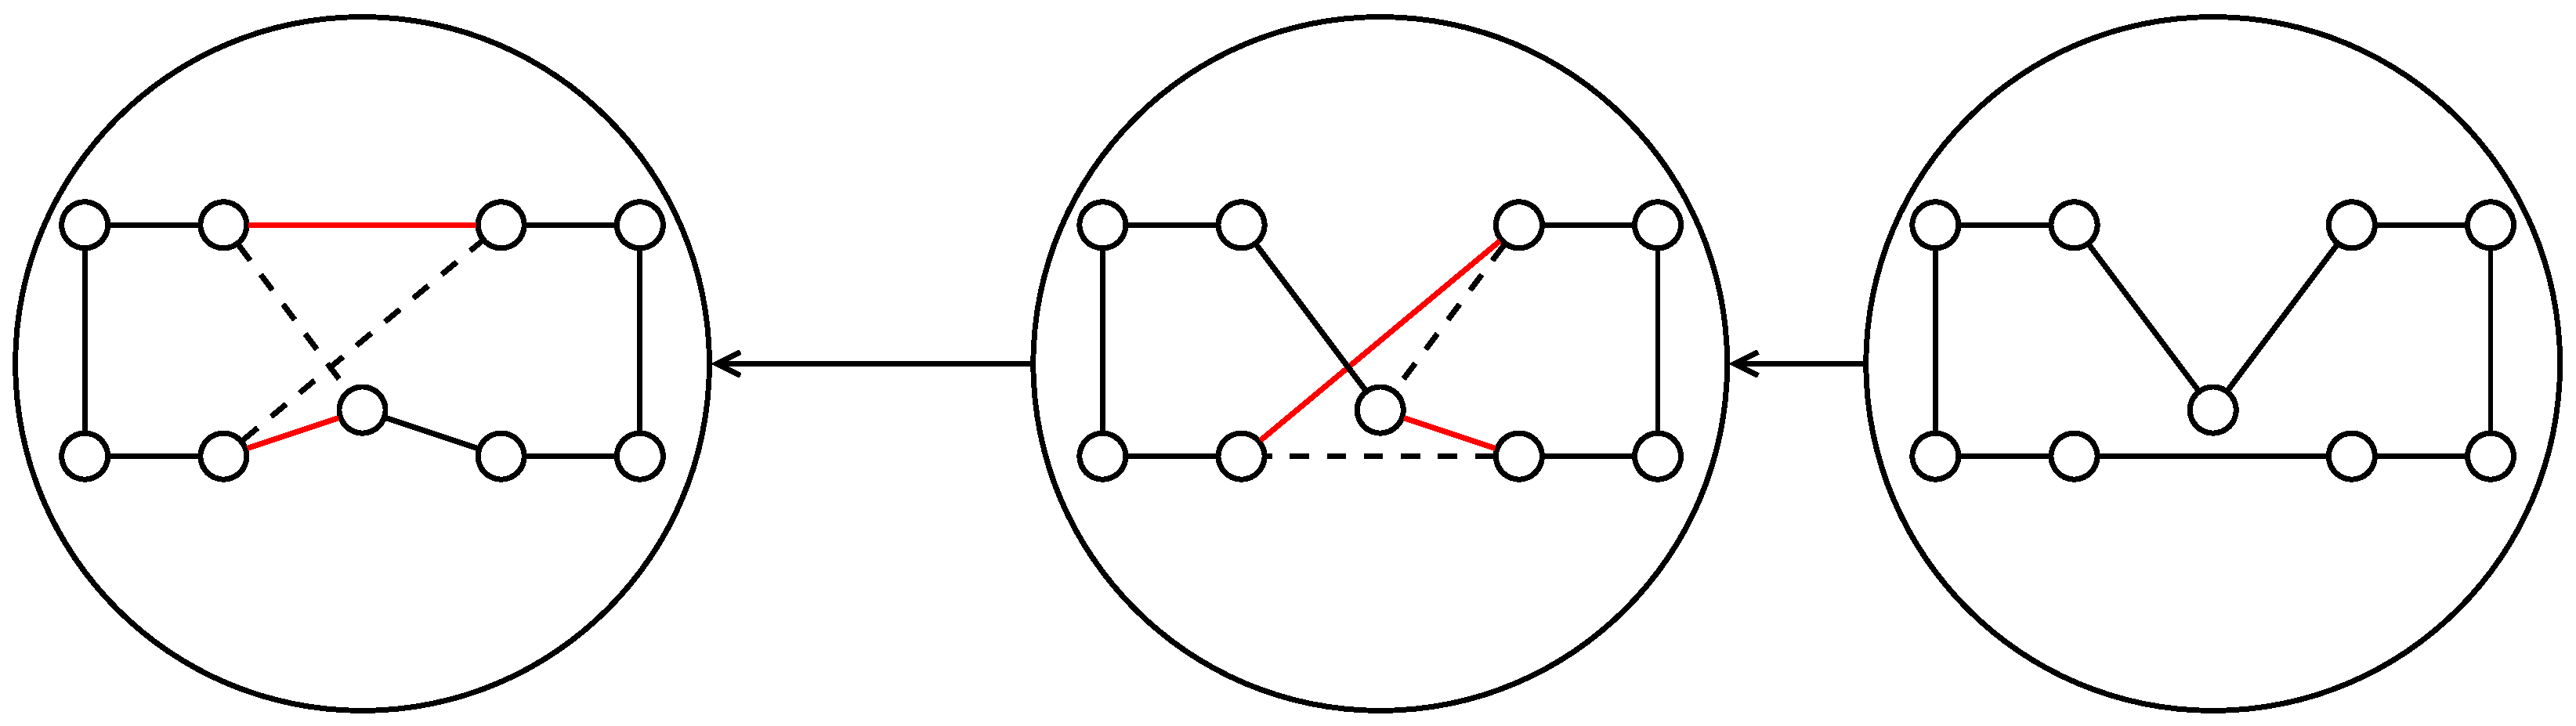
\includegraphics[width=1\linewidth]{Grafik/Aufgabe1}
\caption{Wie in der Vorlesung gezeigt, kann der Graph links nicht weiter durch einen 2-change optimiert werden. Durch den \textit{schlechten} Schritt in der Mitte ist aber die Lösung links zu erreichen.}
\label{fig:Aufgabe1}
\end{figure}
\section*{Aufgabe 2}
\subsection*{a)}
\paragraph{Behauptung}
Seien $T$ und $T'$ Spannbäume in G und $ST_G$ die Menge aller Spannbäume in G.\\
\[ \forall~e\in T\setminus T'~~\exists~e'\in T'\setminus T~|~((T\setminus  \{e\})\cup \{e'\}) \in ST_G \land ((T'\setminus \{e'\})\cup \{e\}) \in ST_G \]
\paragraph{Beweis}
\stepcounter{beweis}
\subparagraph{\Roman{beweis} Behauptung}
Sei $C$ ein beliebiger eindeutiger Kreis.\\
Sei $T$ ein Spannbaum in $G=(V,E)$, wobei $E$ die Kantenmenge von $G$ ist, dann gilt 
\[ \forall~ e'\in E\setminus T ~|~ \exists!~ C\in T\cup \{e'\} \]
\subparagraph{\Roman{beweis} Beweis}
$T$ deckt bereits alle Knoten ab, somit verbindet $e'$ zwei bereits abgedeckte Knoten neu. Da diese schon von jedem Knoten im Graphen erreichbar waren, wurde nun ein Kreis $C$ gebildet.

\begin{flushright}
	q.e.d.
\end{flushright}
\stepcounter{beweis}
\subparagraph{\Roman{beweis} Behauptung}
Sei $T$ ein Spannbaum des Graphen $G$. Sei $C$ die Menge der Knoten, welche an dem Kreis in $T\cup e'$ beteiligt sind. Nun gilt 
\[ \forall~e\in C ~|~ (T\cup \{e'\})\setminus \{e\} =T'\in ST_G \]
\subparagraph{\Roman{beweis} Beweis}
Für alle Knoten in $G$, welche der Kreis $C$ abdeckt gilt, dass genau 2 Pfade von jedem Knoten in $G$ über die Kanten $T\cup \{e'\}$ zu ihnen führen. Wird nun eine Kante $e$ aus $C$ entfernt, so wird lediglich einer dieser Pfade zerstört. Somit existiert genau ein Pfad von jedem Knoten in $G$ über die Kanten $(T\setminus \{e'\})\cup \{e\}$ zu jedem anderen Knoten.\\
$\Rightarrow (T\setminus \{e'\})\cup \{e\}$ ist ein Spannbaum.

\begin{flushright}
	q.e.d.
\end{flushright}
\stepcounter{beweis}
\subparagraph{\Roman{beweis} Behauptung}
Seien $T$ und $T'$ zwei Spannbäume in $G=(V,E)$. Weiter sei $C_X$ ein eindeutiger Kreis in der Knotenmenge $X$. 
\[ \forall~e'\in T'\setminus T~~\exists~e\in C_{(T\cup \{e'\})}\cap (T\setminus T')\]
\subparagraph{\Roman{beweis} Beweis}$ $\\
Annahme: \[C_{(T\cup \{e'\})}\cap (T\setminus T') = \emptyset\]
Widerspruch:
\[ C_{(T\cup \{e'\})}\cap (T\setminus T') = \emptyset~~\land C_{(T\cup \{e'\})} \cap T = C_{(T\cup \{e'\})}\setminus\{ e' \} \Rightarrow C_{(T\cup \{e'\})}\setminus\{ e' \}\subseteq T' \land \{ e' \} \subseteq T'\]
\[ \Rightarrow(C_{(T\cup \{e'\})}\setminus\{ e' \})\cup \{e'\} = C_{(T\cup \{e'\})} \subseteq T' \lightning \]
Da $T'$ nach Annahme ein Spannbaum ist, und als solcher keinen Kreis beinhalten kann.\\
$\Rightarrow $
\[ \forall~e'\in T'\setminus T~~\exists~e\in C_{(T\cup \{e'\})}\cap (T\setminus T') \]

\begin{flushright}
	q.e.d.
\end{flushright}
\paragraph{Beweis (Fortsetzung)}$ $\\
Aus I
\[ \forall~ e'\in E\setminus T ~|~ \exists!~ C\in T\cup \{e'\} \]
Aus II
\[ \forall~e\in C ~|~ (T\cup \{e'\})\setminus \{e\} =T'\in ST_G \]
Aus III
\[ \forall~e'\in T'\setminus T~~\exists~e\in C_{(T\cup \{e'\})}\cap (T\setminus T')\]

Aus I folgt, dass durch das hinzufügen einer neuen Kante in einen Spannbaum in diesem ein Kreis gebildet wird.\\
Aus II folgt, dass wenn man aus diesem Kreis eine beliebige Kante entfernt ein neuer  Spannbaum entsteht.\\
Aus III folgt, dass wenn man einem Spannbaum $T$ eine neue Kante $e'$ aus $T'$ hinzufügt, es auch eine Kante in $T$ geben muss, welche nicht in $T'$ ist, aber in dem durch $e'$ erzeugten Kreis.\\

Aus I folgt, dass in den in der Behauptung genannten Kantenmengen $T^*:=(T\setminus\{e\})\cup\{e'\}$ und $T'^*:= (T'\setminus\{e'\})\cup\{e\}$ 
durch $T\cup \{e'\}$ und $T' \cup \{e\}$ jeweils ein Kreis gebildet wird.
Aus III folgt, dass die Kante $e'$ so existiert, dass durch II $T^*$ und $T'^*$ wieder Spannbäume sind.
\begin{flushright}
	q.e.d.
\end{flushright}

\subsection*{b)}
Nach dem Lemma aus Aufgabe a) kann man eine Kante e aus $T$ mit einer Kante e' aus $T'$ tauschen, so dass ein neuer Spannbaum entsteht. Seien 
\[T_i:= T_{i-1}.swap(e,e') | i\in\{1,\ldots,k\},~e\in T_{i-1}\setminus T',~ e'\in T'\setminus T_{i-1}~~T_0=T\]
 die Spannbäume, welche nach i Schritten entstehen. Weiter gilt $|T\setminus T'| - i = |T_i\setminus T'|$, da mit jedem Schritt sich der Spannbaum $T_i$ dem Spannbaum $T'$ annähert. Sobald $i = |T\setminus T'|$ folgt $T_i = T'$, da sich keine Kante mehr unterscheidet. Die maximale Anzahl an Schritten ist somit $|T\setminus T'| \leq n-1$, da sie sich höchstens um $n-1$ Kanten, bei 2 Spannbäumen mit disjunkten Kantenmengen, unterscheiden können.
\end{document}

